\documentclass[aspectratio=169]{beamer}
\usetheme{Madrid}
\usepackage{graphicx,booktabs,array}
\title[Bina.az Price Prediction]{Bina.az Housing Price Prediction}
\subtitle{From-scratch decision trees and Pegasos SVM}
\author[PegaSold]{PegaSold\\[.35em]Emiliya Abdulhalimova · Aygun Asvarova · Murad Bagirzade · Kanan Karimli}
\institute[MLE-AI-201]{MLE-AI-201 Final Project V3 · National AI Center}
\date[Oct 2026]{October 2026}
\begin{document}
\begin{frame}\titlepage\end{frame}
\section{Project and data}
\begin{frame}{Project question — Speaker 1: data and task}
\begin{itemize}
\item Real Bina.az asking-price scrape: 100,775 raw rows from October–November 2024.
\item Task A predicts $\ln(\mathrm{price})$; we report log-space and AZN-space errors.
\item Task B classifies standard vs premium; the training median cutoff is 208,000 AZN.
\item The decision tree and Pegasos are NumPy implementations; sklearn is used as a comparison reference.
\end{itemize}
\end{frame}
\begin{frame}{Cleaning and leakage — Speaker 1}
\small
\begin{columns}[T]\column{.47\textwidth}
\begin{itemize}
\item Keep the latest scrape per normalized advert ID; retain Baku residential listings.
\item Apply declared price, area, AZN/m$^2$, room and floor checks.
\item Train-only log-price MAD fence: 26,130–1,671,651 AZN; removed 246 train rows only.
\item Split: 40,033/8,632/8,632; validation/test rows remain intact.
\item Exclude target-derived prices, free text, identifiers, seller fields and raw address.
\item Fit imputation, scaling and category vocabulary from training rows.
\end{itemize}
\column{.53\textwidth}\centering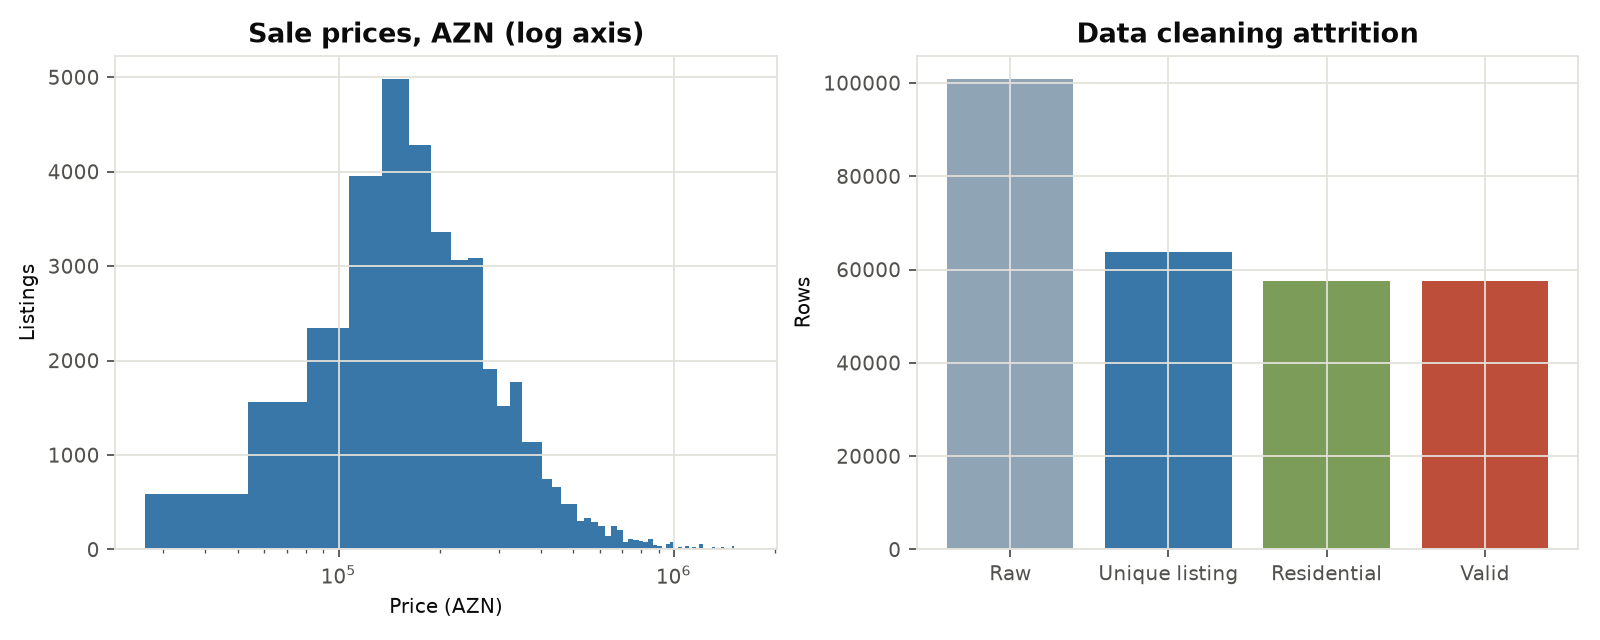
\includegraphics[width=\linewidth,height=.74\textheight,keepaspectratio]{../reports/figures/data_and_prices.png}\end{columns}
\end{frame}
\begin{frame}{Exploration and feature design — Speaker 1}
\small
\begin{columns}[T]\column{.47\textwidth}
\begin{itemize}
\item Parse Azerbaijani measurements; encode flags as 0/1.
\item Use area, rooms, floor, land, coordinates, category and frequent locations.
\item Engineer distance to centre, floor ratio, area per room and land ratio.
\item Spatial and property-type patterns provide signal, not causal proof.
\item This is a historical asking-price scrape, not transaction data.
\end{itemize}
\column{.51\textwidth}\centering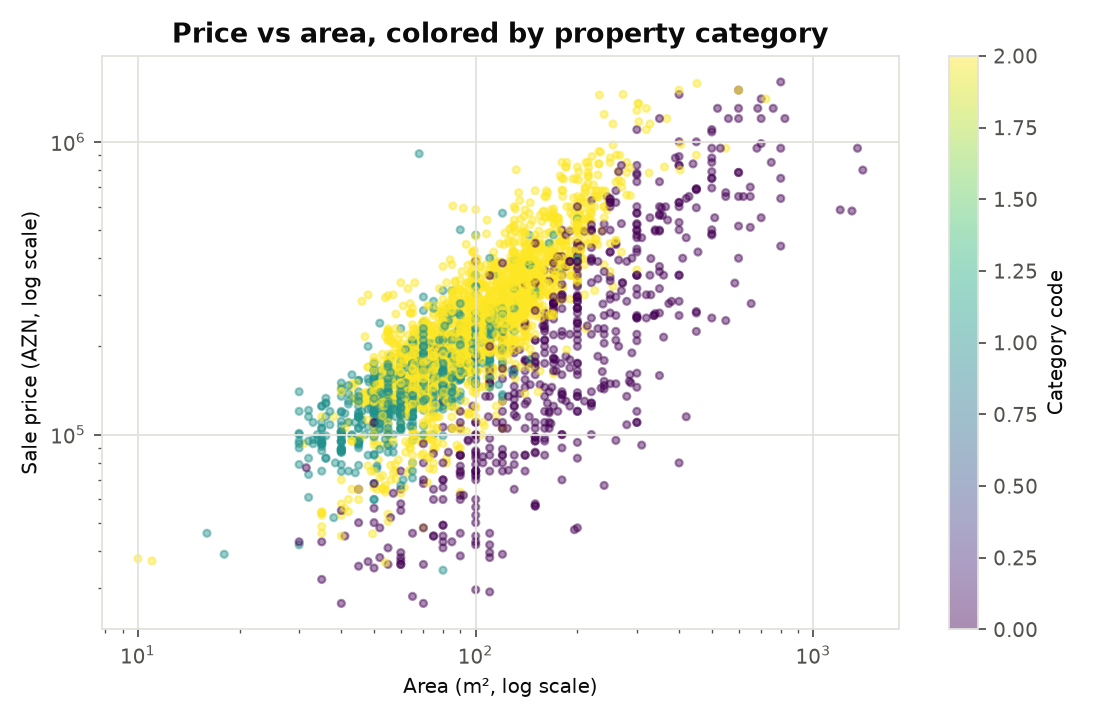
\includegraphics[width=\linewidth,height=.73\textheight,keepaspectratio]{../reports/figures/price_vs_area.png}\end{columns}
\end{frame}
\begin{frame}{Split protocol and cross-validation — Speaker 1}
\begin{itemize}
\item Fixed seed; split allocation balances price bins and keeps repeated advert IDs together.
\item Premium threshold is computed from training prices only: 208,000 AZN.
\item Validation chooses hyperparameters; the held-out test is used after selection.
\item Five-fold CV uses all 40,033 training rows (about 32k fit / 8k validation per fold).
\item Preprocessing statistics were fitted before folds; CV is indicative, not fully nested.
\end{itemize}
\end{frame}
\section{Models}
\begin{frame}{Decision tree from scratch — Speaker 2}
\small
\begin{columns}[T]\column{.48\textwidth}
\begin{itemize}
\item Sort numeric values and test boundaries between distinct adjacent values.
\item Classification: Gini/entropy information gain; regression: MSE reduction.
\item Cumulative counts and sums make split scoring efficient.
\item Leaves predict majority class or mean target.
\item Depth and minimum-leaf limits control model variance.
\item Validation selects criterion, depth and leaf size; test remains untouched.
\end{itemize}
\column{.50\textwidth}\centering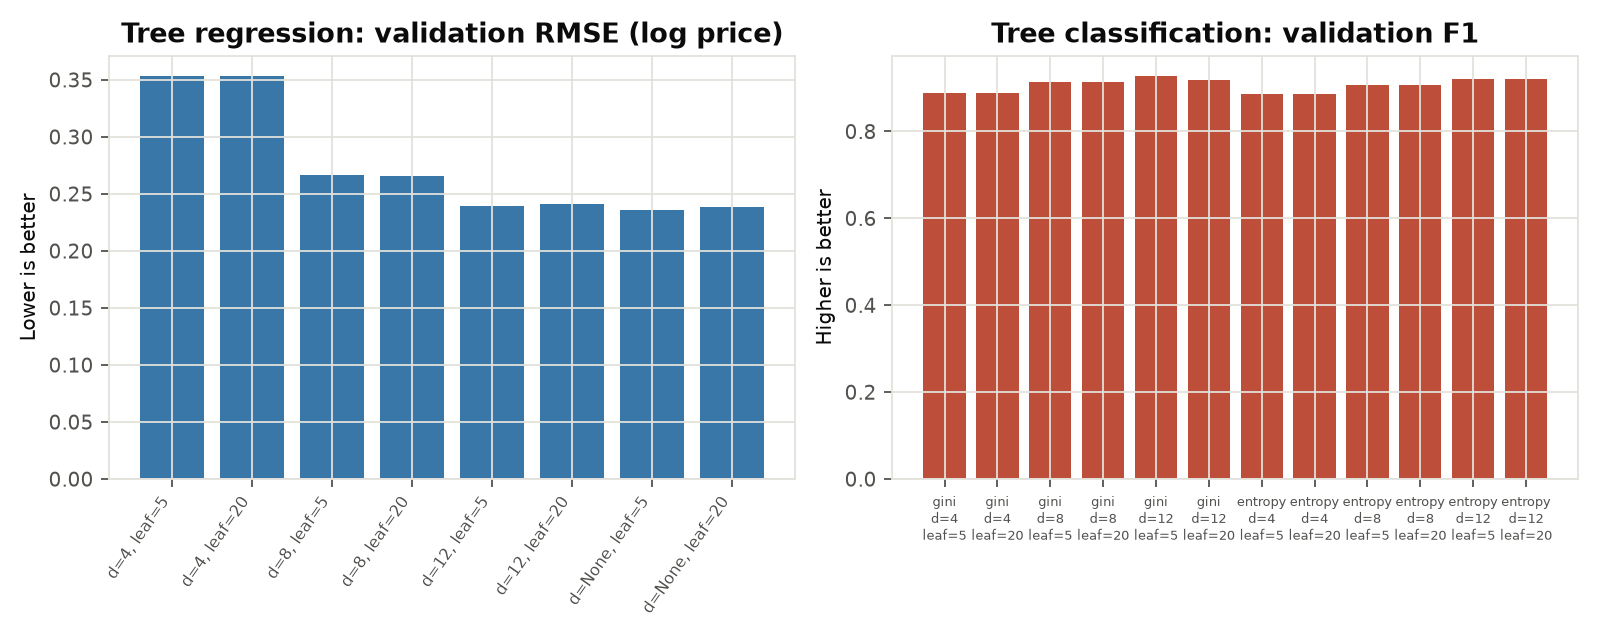
\includegraphics[width=\linewidth,height=.71\textheight,keepaspectratio]{../reports/figures/tree_tuning.png}\end{columns}
\end{frame}
\begin{frame}{Tree results and generalization — Speaker 2}
\centering\small
\begin{tabular*}{.92\linewidth}{@{\extracolsep{\fill}}lrlr}
\toprule Metric & Score & Metric & Score\\\midrule
Task A log RMSE & 0.239 & Task B accuracy & 0.922\\
Task A AZN RMSE & 147,356 & Task B F1 / AUC & 0.923 / 0.958\\
Reference log RMSE & 0.239 & Reference accuracy & 0.922\\
\bottomrule\end{tabular*}
\vspace{.15cm}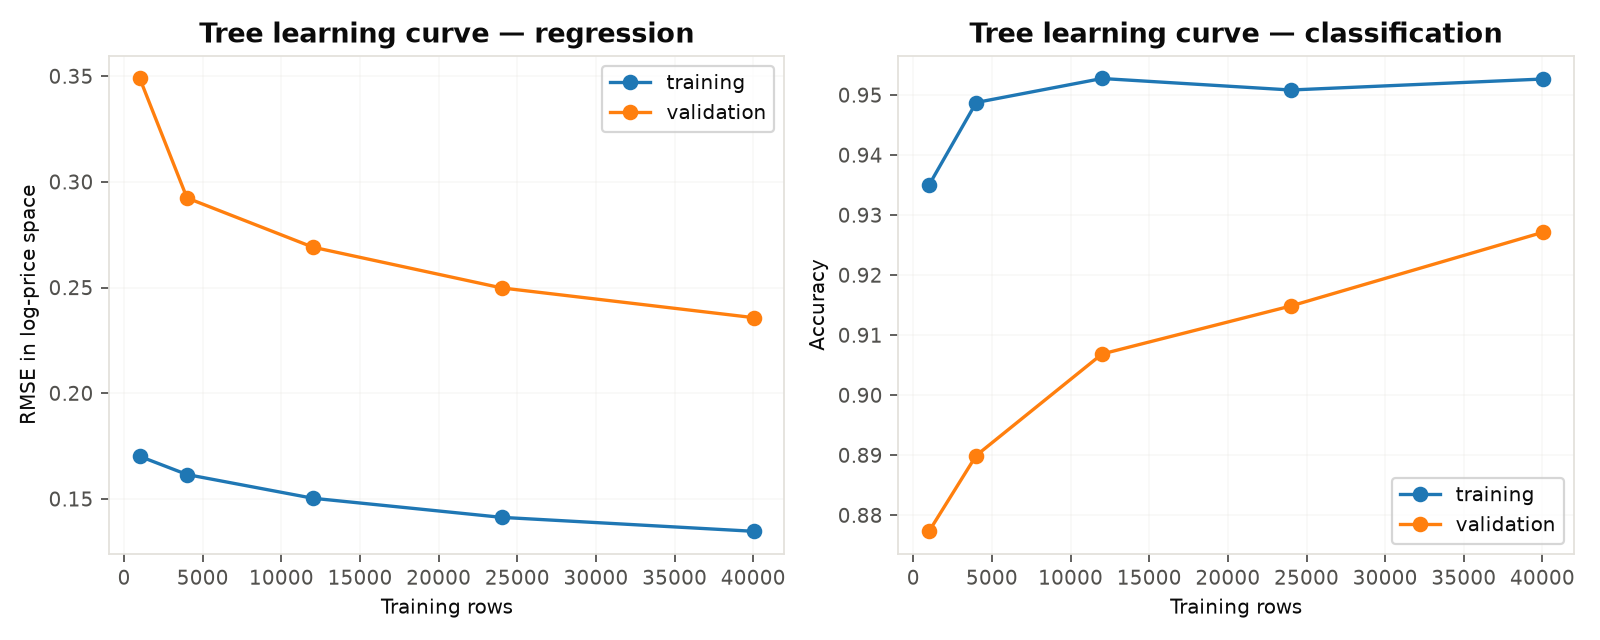
\includegraphics[width=.89\linewidth,height=.51\textheight,keepaspectratio]{../reports/figures/tree_learning_curves.png}
\end{frame}
\begin{frame}{Regression error in AZN — Speaker 2}
\small
\begin{columns}[T]\column{.43\textwidth}
\begin{itemize}
\item Held-out test MAE: 47,613 AZN; median absolute error: 16,431 AZN.
\item Test RMSE: 147,356 AZN.
\item Largest absolute error: 3,760,714 AZN.
\item Actual 5,000,000 AZN; predicted 1,239,286 AZN.
\item Test retains extreme prices outside the training MAD fence.
\end{itemize}
\column{.55\textwidth}\centering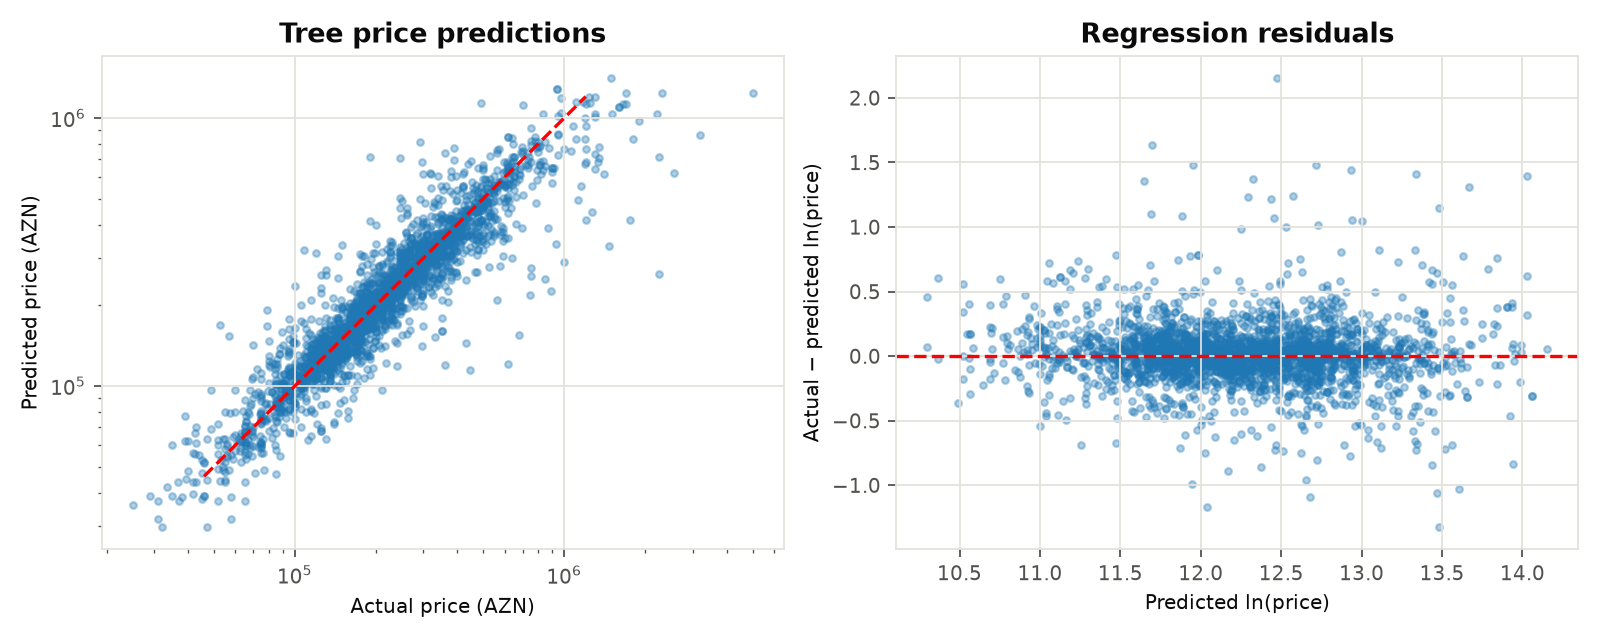
\includegraphics[width=\linewidth,height=.73\textheight,keepaspectratio]{../reports/figures/regression_error_analysis.png}\end{columns}
\end{frame}
\begin{frame}{Linear Pegasos SVM — Speaker 3}
\small
\begin{columns}[T]\column{.50\textwidth}
\begin{itemize}
\item Minimize regularized hinge loss with stochastic sub-gradient updates.
\item Standardize using training data; labels map to $-1,+1$.
\item Selected $\lambda=0.01$; margin width $2/\|w\|=0.900$.
\item Support vectors (signed margin $\leq1$): 11,587 training rows.
\item Test accuracy 0.902; F1 0.903; ROC-AUC 0.968.
\end{itemize}
\column{.48\textwidth}\centering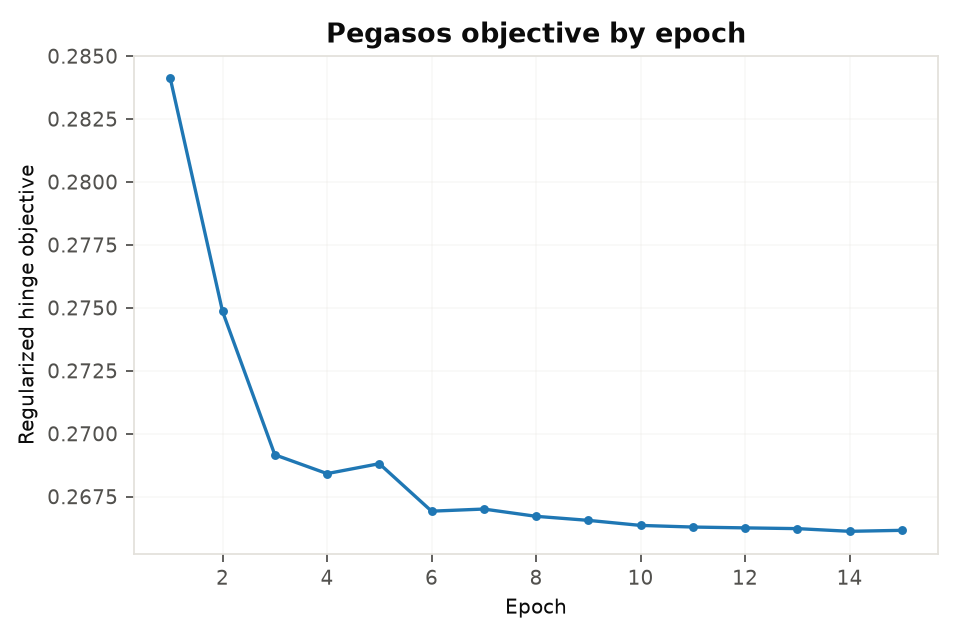
\includegraphics[width=\linewidth,height=.76\textheight,keepaspectratio]{../reports/figures/pegasos_objective.png}\end{columns}
\end{frame}
\begin{frame}{Nonlinear SVM and decision margin — Speaker 3}
\small
\begin{columns}[T]\column{.48\textwidth}
\begin{itemize}
\item Seeded Random Fourier Features approximate an RBF kernel; the NumPy Pegasos optimizer trains the mapped features.
\item 128 components; selected $\gamma=0.01$; training subset 8,000.
\item Matched RBF SVC uses the same subset; results depend on random features and seed.
\item Nonlinear mapping did not outperform the linear model in this run.
\end{itemize}
\column{.50\textwidth}\centering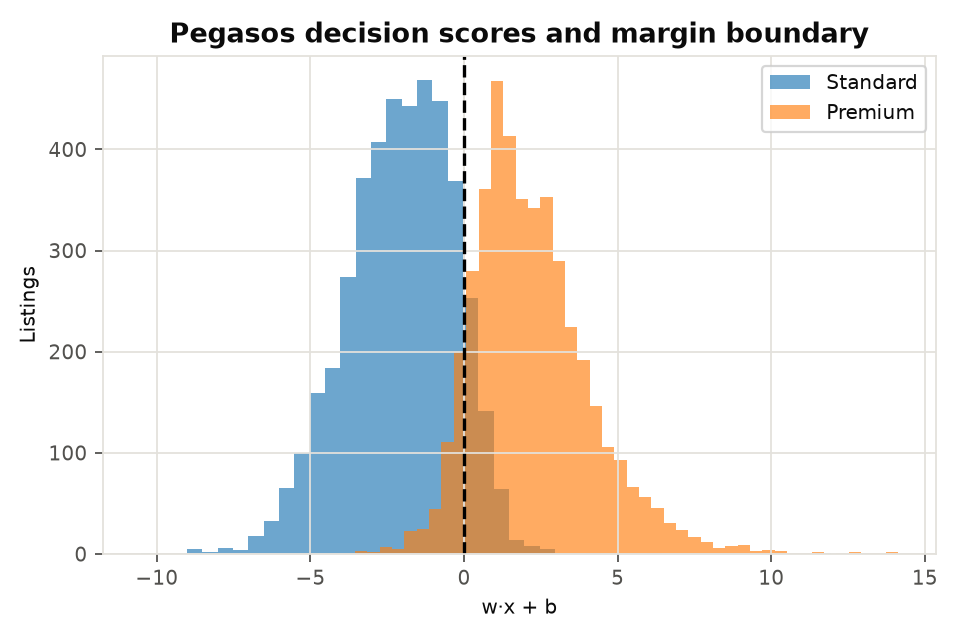
\includegraphics[width=\linewidth,height=.76\textheight,keepaspectratio]{../reports/figures/svm_margin_scores.png}\end{columns}
\end{frame}
\section{Evaluation and findings}
\begin{frame}{Fair comparison and uncertainty — Speaker 4}
\small
\begin{columns}[T]\column{.49\textwidth}
\begin{itemize}
\item Tree references use matched criteria, depth and leaf settings.
\item LinearSVC uses hinge loss, fold-local scaling and objective-matched $C=1/(\lambda n)$.
\item Five-fold CV covers all 40,033 training rows.
\item Regression tree CV MAE: 41,505 $\pm$ 675 AZN.
\item sklearn tree CV MAE: 41,516 $\pm$ 696 AZN.
\item CV MAE is lower partly because filtered folds do not contain the test's full extreme-price tail.
\end{itemize}
\column{.49\textwidth}\centering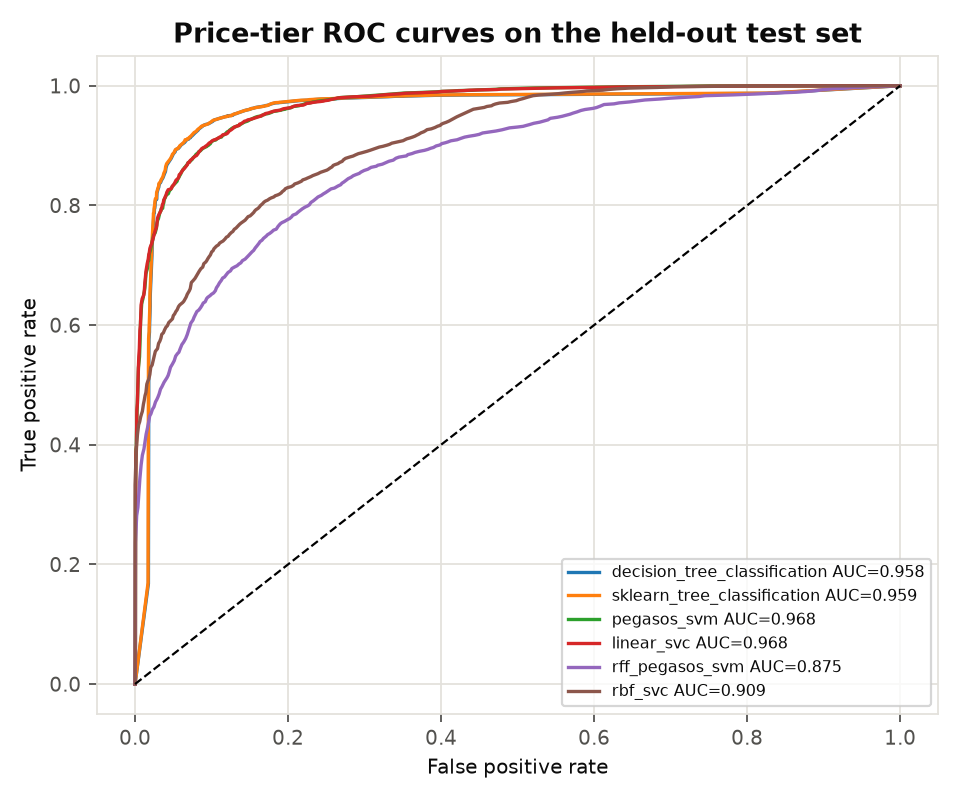
\includegraphics[width=\linewidth,height=.74\textheight,keepaspectratio]{../reports/figures/roc_curves.png}\end{columns}
\end{frame}
\begin{frame}{Held-out test comparison — Speaker 4}
\scriptsize
\begin{tabular*}{\textwidth}{@{\extracolsep{\fill}}lrrrr}
\toprule Model & Accuracy & F1 & AUC & Fit sec\\\midrule
Scratch tree & 0.922 & 0.923 & 0.958 & 1.76\\
sklearn tree & 0.922 & 0.923 & 0.959 & 0.24\\
Pegasos & 0.902 & 0.903 & 0.968 & 2.81\\
LinearSVC & 0.902 & 0.903 & 0.968 & 0.48\\
RFF Pegasos & 0.790 & 0.786 & 0.875 & 0.82\\
\bottomrule\end{tabular*}
\vspace{.18cm}\begin{columns}\column{.5\textwidth}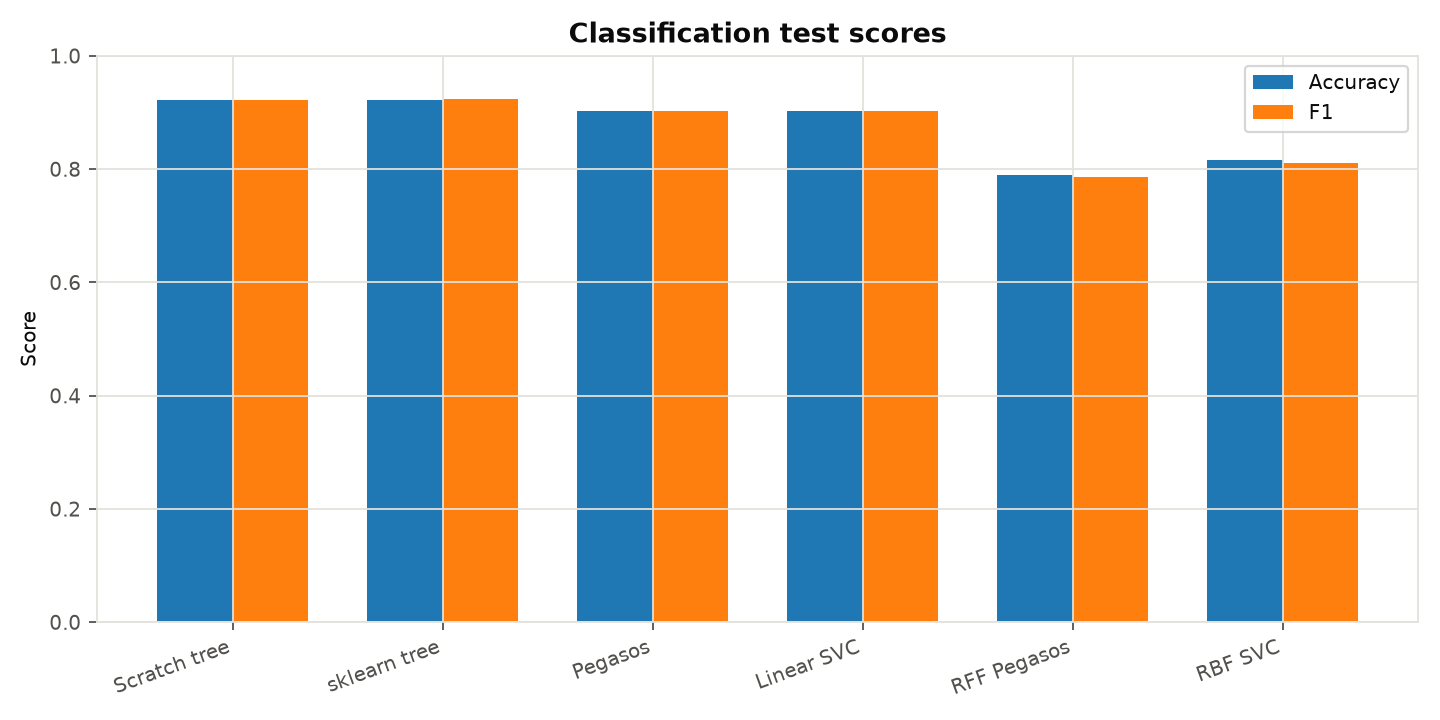
\includegraphics[width=\linewidth,height=.52\textheight,keepaspectratio]{../reports/figures/classification_comparison.png}\column{.5\textwidth}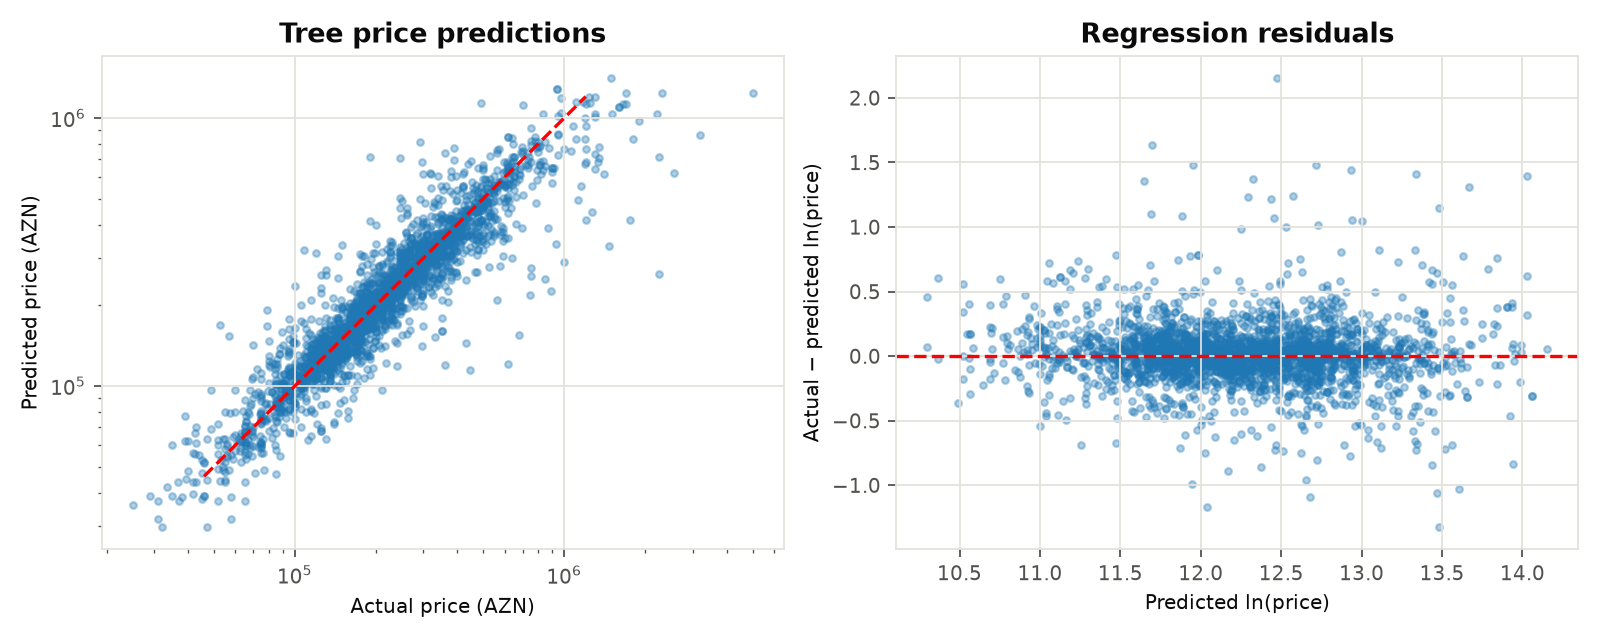
\includegraphics[width=\linewidth,height=.52\textheight,keepaspectratio]{../reports/figures/regression_error_analysis.png}\end{columns}
\end{frame}
\begin{frame}{Tuning and feature importance — Speaker 4}
\begin{columns}[T]\column{.49\textwidth}\centering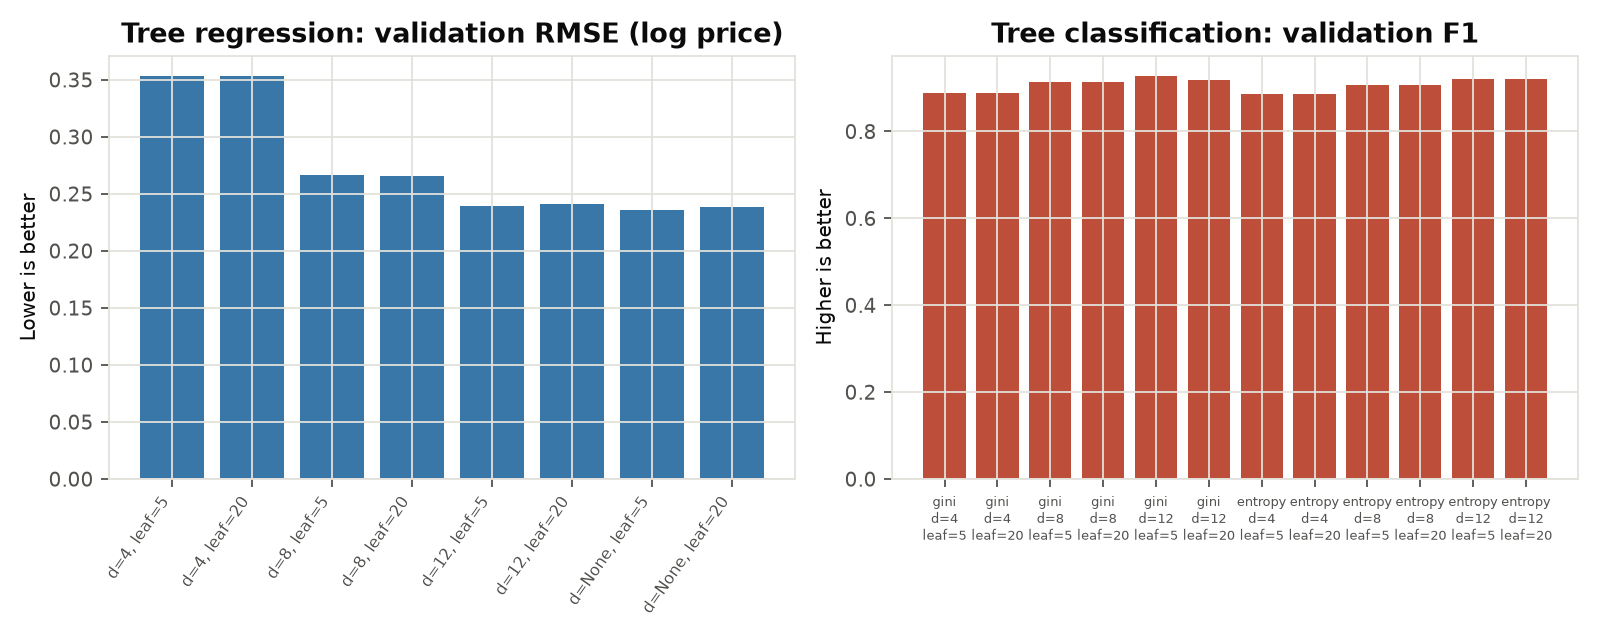
\includegraphics[width=\linewidth,height=.72\textheight,keepaspectratio]{../reports/figures/tree_tuning.png}\\Validation sweeps.
\column{.49\textwidth}\centering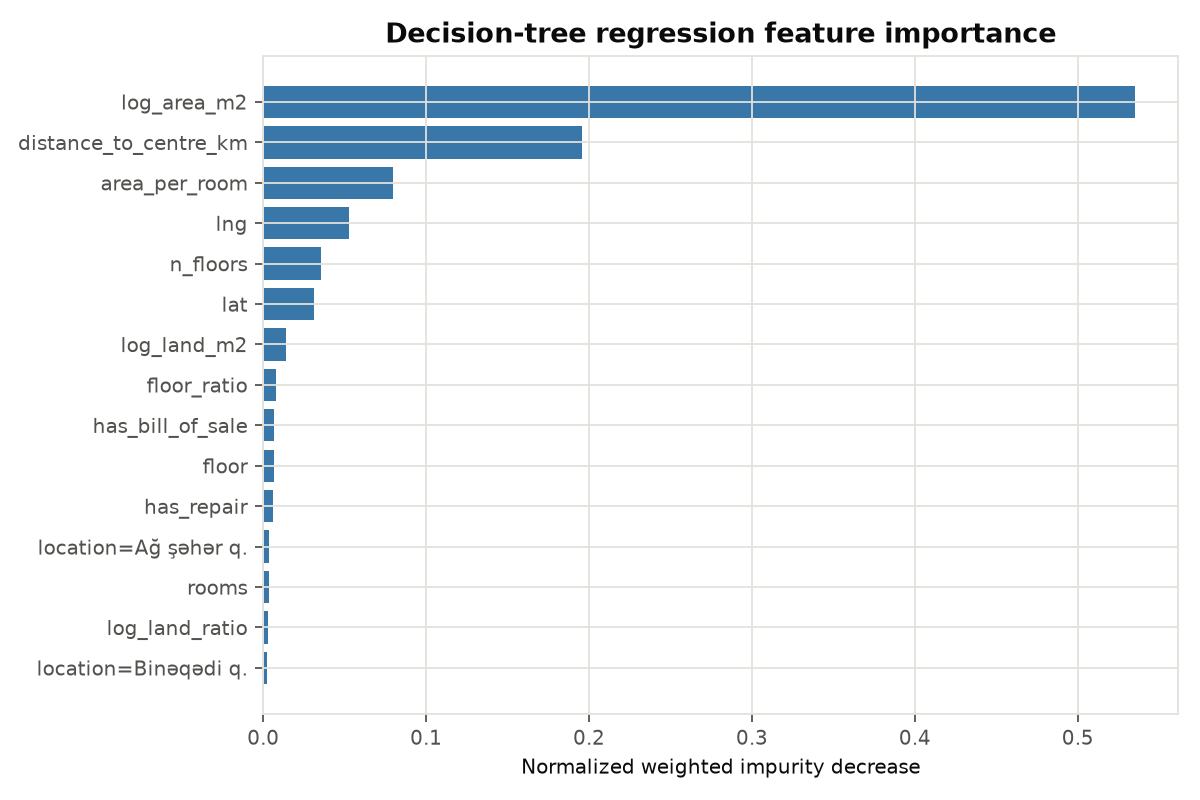
\includegraphics[width=\linewidth,height=.72\textheight,keepaspectratio]{../reports/figures/feature_importance_regression.png}\\Impurity importance is descriptive, not causal.
\end{columns}
\end{frame}
\begin{frame}{Conclusions and limitations — All}
\begin{itemize}
\item Price-tier classification is easier than exact advertised-price prediction; luxury-tail errors remain large.
\item Scratch and sklearn trees are close under matched settings.
\item The held-out test MAE is 47,613 AZN; CV mean does not replace this result.
\item Asking prices are not verified transactions; one 2024 scrape is not today's market.
\item CV preprocessing precedes folds; ambiguous cross-ID duplicates may remain.
\end{itemize}
\end{frame}
\begin{frame}{Reproducibility and handoff — All}
\small
\begin{enumerate}
\item Speaker 1: data preparation, EDA, feature design and split protocol.
\item Speaker 2: NumPy tree, validation tuning and regression error analysis.
\item Speaker 3: Pegasos optimization, margin and nonlinear RFF model.
\item Speaker 4: sklearn benchmarks, CV, metrics and reproducibility.
\end{enumerate}
\begin{block}{Reproduce}
\texttt{python -m src.run\_all}\qquad\texttt{pytest -q}\\
Results, figures and caveats: \texttt{reports/final\_report.md}.
\end{block}
AI assistance was used for coding suggestions, debugging, corrections and review; the team checked the final code and results.
\end{frame}
\end{document}
